\section{Method}
\label{sec:method}

\begin{figure}[t]
\centering
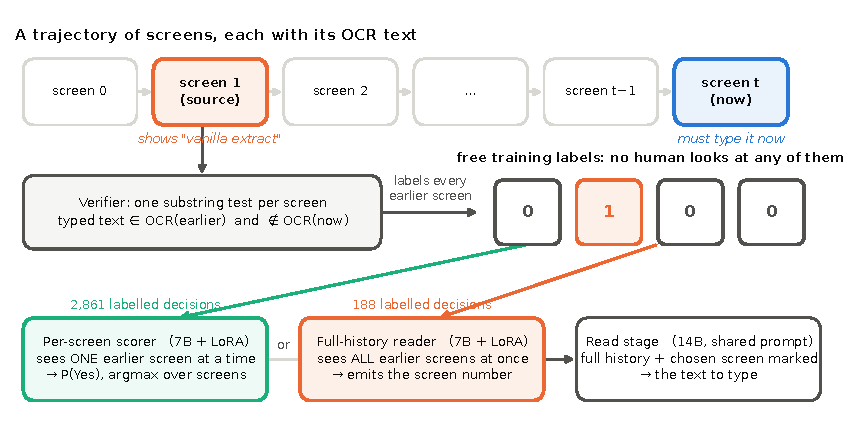
\includegraphics[width=\linewidth]{figures/fig1_method.pdf}
\caption{The verifier does two jobs. Reading left to right along the trajectory, it mines the case: the text typed at step $t$ appears in the OCR of screen 1 and not on screen $t$. Applied to every earlier screen instead of stopping at the first hit, the same test labels all $t$ candidates. Those labels train two instantiations that differ in how the history reaches the model, and therefore in how many decisions one label set yields.}
\label{fig:method}
\end{figure}

\subsection{A string check both finds and labels the needs}
\label{sec:needs}
A step $t$ has a delayed information need when the text the agent types at $t$ appears verbatim in the OCR text of an earlier screen $i<t$ and does not appear on screen $t$. The gap is $t-i$ for the latest such $i$. The second clause is load-bearing: when the text is on the current screen the agent needs no memory at all, and Section~\ref{sec:index} shows that keeping those steps rewards any method that reads recent screens.

A candidate is any TYPE action whose argument has three or more characters and does not occur in the task description; we normalize strings by lower-casing and stripping whitespace and punctuation. We run EasyOCR on every screenshot of the sampled trajectories and test the argument against earlier screens and the current one. In the first sample of 300 GUI-Odyssey trajectories, 127 of 431 candidates pass the OCR check (269 fail, most of them OCR misreads on inspection, and 35 lack OCR output). Removing 36 whose text is also on the current screen leaves 91 verified cases; removing 6 whose text appears in the task's step-by-step instruction field leaves 85. The verifier also returns the full set of screens containing the text, which is the label.

\begin{table}[t]
\centering\footnotesize\setlength{\tabcolsep}{4pt}
\caption{AITZ's 7.4-step tasks contain no delayed information need; GUI-Odyssey's 15.4-step tasks contain one in 31\% of sampled trajectories. We mine only the sampled trajectories.}
\label{tab:prev}
\resizebox{\linewidth}{!}{%
\begin{tabular}{lrrrl}
\toprule
 & trajectories & steps & mean length & verified delayed needs \\
\midrule
AITZ~\citep{aitz} & 2,504 & 18,643 & 7.4 & 0 \\
GUI-Odyssey~\citep{guiodyssey} (full) & 7,735 & 118,791 & 15.4 & not mined \\
\quad sampled, complete OCR & 273 & 4,338 & 15.9 & 89 steps (2.05\%); 31\% of trajectories \\
\bottomrule
\end{tabular}}
\end{table}

Table~\ref{tab:prev} gives the prevalence. The need is also far and inconspicuous: the gap has median 5 and maximum 27 screens, 56\% of gaps are 5 or more, and on its source screen the needed text sits at a median rank of 13 among 33 OCR elements and is never first. A one-line summary that keeps the few most prominent elements therefore cannot be expected to retain it.

\paragraph{Four samples.} The \emph{short set} holds the 85 cases above (need step index $t$, median 11). The \emph{long set} holds 53 cases with $t\ge16$ from a second sample of 300 trajectories of $\ge20$ steps (127 before the current-screen filter, all 74 removals being leakage). The \emph{late-mined set} holds 50 cases with $t\ge16$ from a third sample of 200 trajectories. These three give 188 cases in 170 trajectories and carry all training and cross-validation. The \emph{external set} holds 93 cases from a fourth sample of 400 trajectories of $\ge16$ steps, mined after every design decision was fixed and evaluated once.

\subsection{Two instantiations, one label set}
Each verified case $(e,t)$ yields one training item per earlier screen $i<t$. For the \textbf{per-screen scorer} the item is a pair: the input holds the task description, the OCR text of screen $t$, the OCR text of screen $i$ and the distance $t-i$, and the label is 1 if $i$ is in the verifier's set. The 188 cases yield 2,861 pairs, 463 of them positive. For the \textbf{full-history reader} the item is one example per case: the input holds the task and every earlier screen, and the target is the number of the latest screen in the verifier's set. No human labels any item.

The scorer is Qwen2.5-7B-Instruct~\citep{qwen25} with a LoRA~\citep{lora} adapter of rank 16 on the attention projections (40M trainable parameters). Its prompt ends with ``Answer Yes or No''; we take the logits of \texttt{Yes} and \texttt{No} at the answer position, apply a two-way softmax, and minimize cross-entropy with positives weighted 3 to 1. Localization is the argmax of $P(\text{Yes})$ over earlier screens, computed by $t$ forward passes of 600--900 tokens each and no generation. The full-history reader uses the same base model and adapter rank, fine-tuned to emit the screen number with the loss on the number only; localization is one greedy generation of at most five tokens. Both train for 2 epochs at learning rate $10^{-4}$ with 4 items per update, 13--27 minutes per fold on one 48GB GPU.

\paragraph{Read stage.} A Qwen2.5-14B-Instruct reader then types the text, with the prompt shared by every condition. \emph{Single-screen read} receives the task, the current screen and the chosen screen's OCR text. \emph{Read with history} receives the full history as well, with the chosen screen repeated and marked before the current screen; it costs full history's context plus one repeated screen.

\paragraph{Cost.} At $t=16$ the scorer reads about 12K tokens across $t$ small forward passes, while the full-history reader and prompted full history read 1--5K tokens in one pass. A 3B scorer loses 4.2 points overall and gains 11.1 at $t\ge20$ (Section~\ref{sec:ablation}), so the scorer's cost is adjustable.

\paragraph{Protocol.} We split the 188 cases into five folds, keeping every case from one trajectory in the same fold so no trajectory appears in both train and test. We train on four folds, score the fifth, and pool the five scored folds; every cross-validated number below is that pool. For the external set we train once on all 188 cases and evaluate once. Localization is correct when the named screen is any screen whose OCR contains the gold text (\emph{any-valid scoring}); end-to-end is correct when the produced text, normalized as in mining, contains the gold text. All comparisons are paired on the same cases and tested with McNemar's test; we report the net number of cases that flip and the two-sided $p$.
